\documentclass{recipe}

\begin{document}
\begin{recipe}{Pork Noodles}
  \servings{2}

  \begin{ingredients}
    \ingredient{1}{in}{pork chop}
    \ingredient{}{}{salt}
    \ingredient{8}{oz}{egg noodles}
    \ingredient{}{}{herbs de provence}
    \ingredient{}{}{flour}
    \ingredient{1}{tbsp}{butter}
    \ingredient{2}{tbsp}{apple juice}
    \ingredient{}{}{pepper}
    \ingredient{1}{egg}
    \ingredient{1/8}{cup}{mild cheddar cheese}
  \end{ingredients}

  \begin{images}
    \begin{image}
      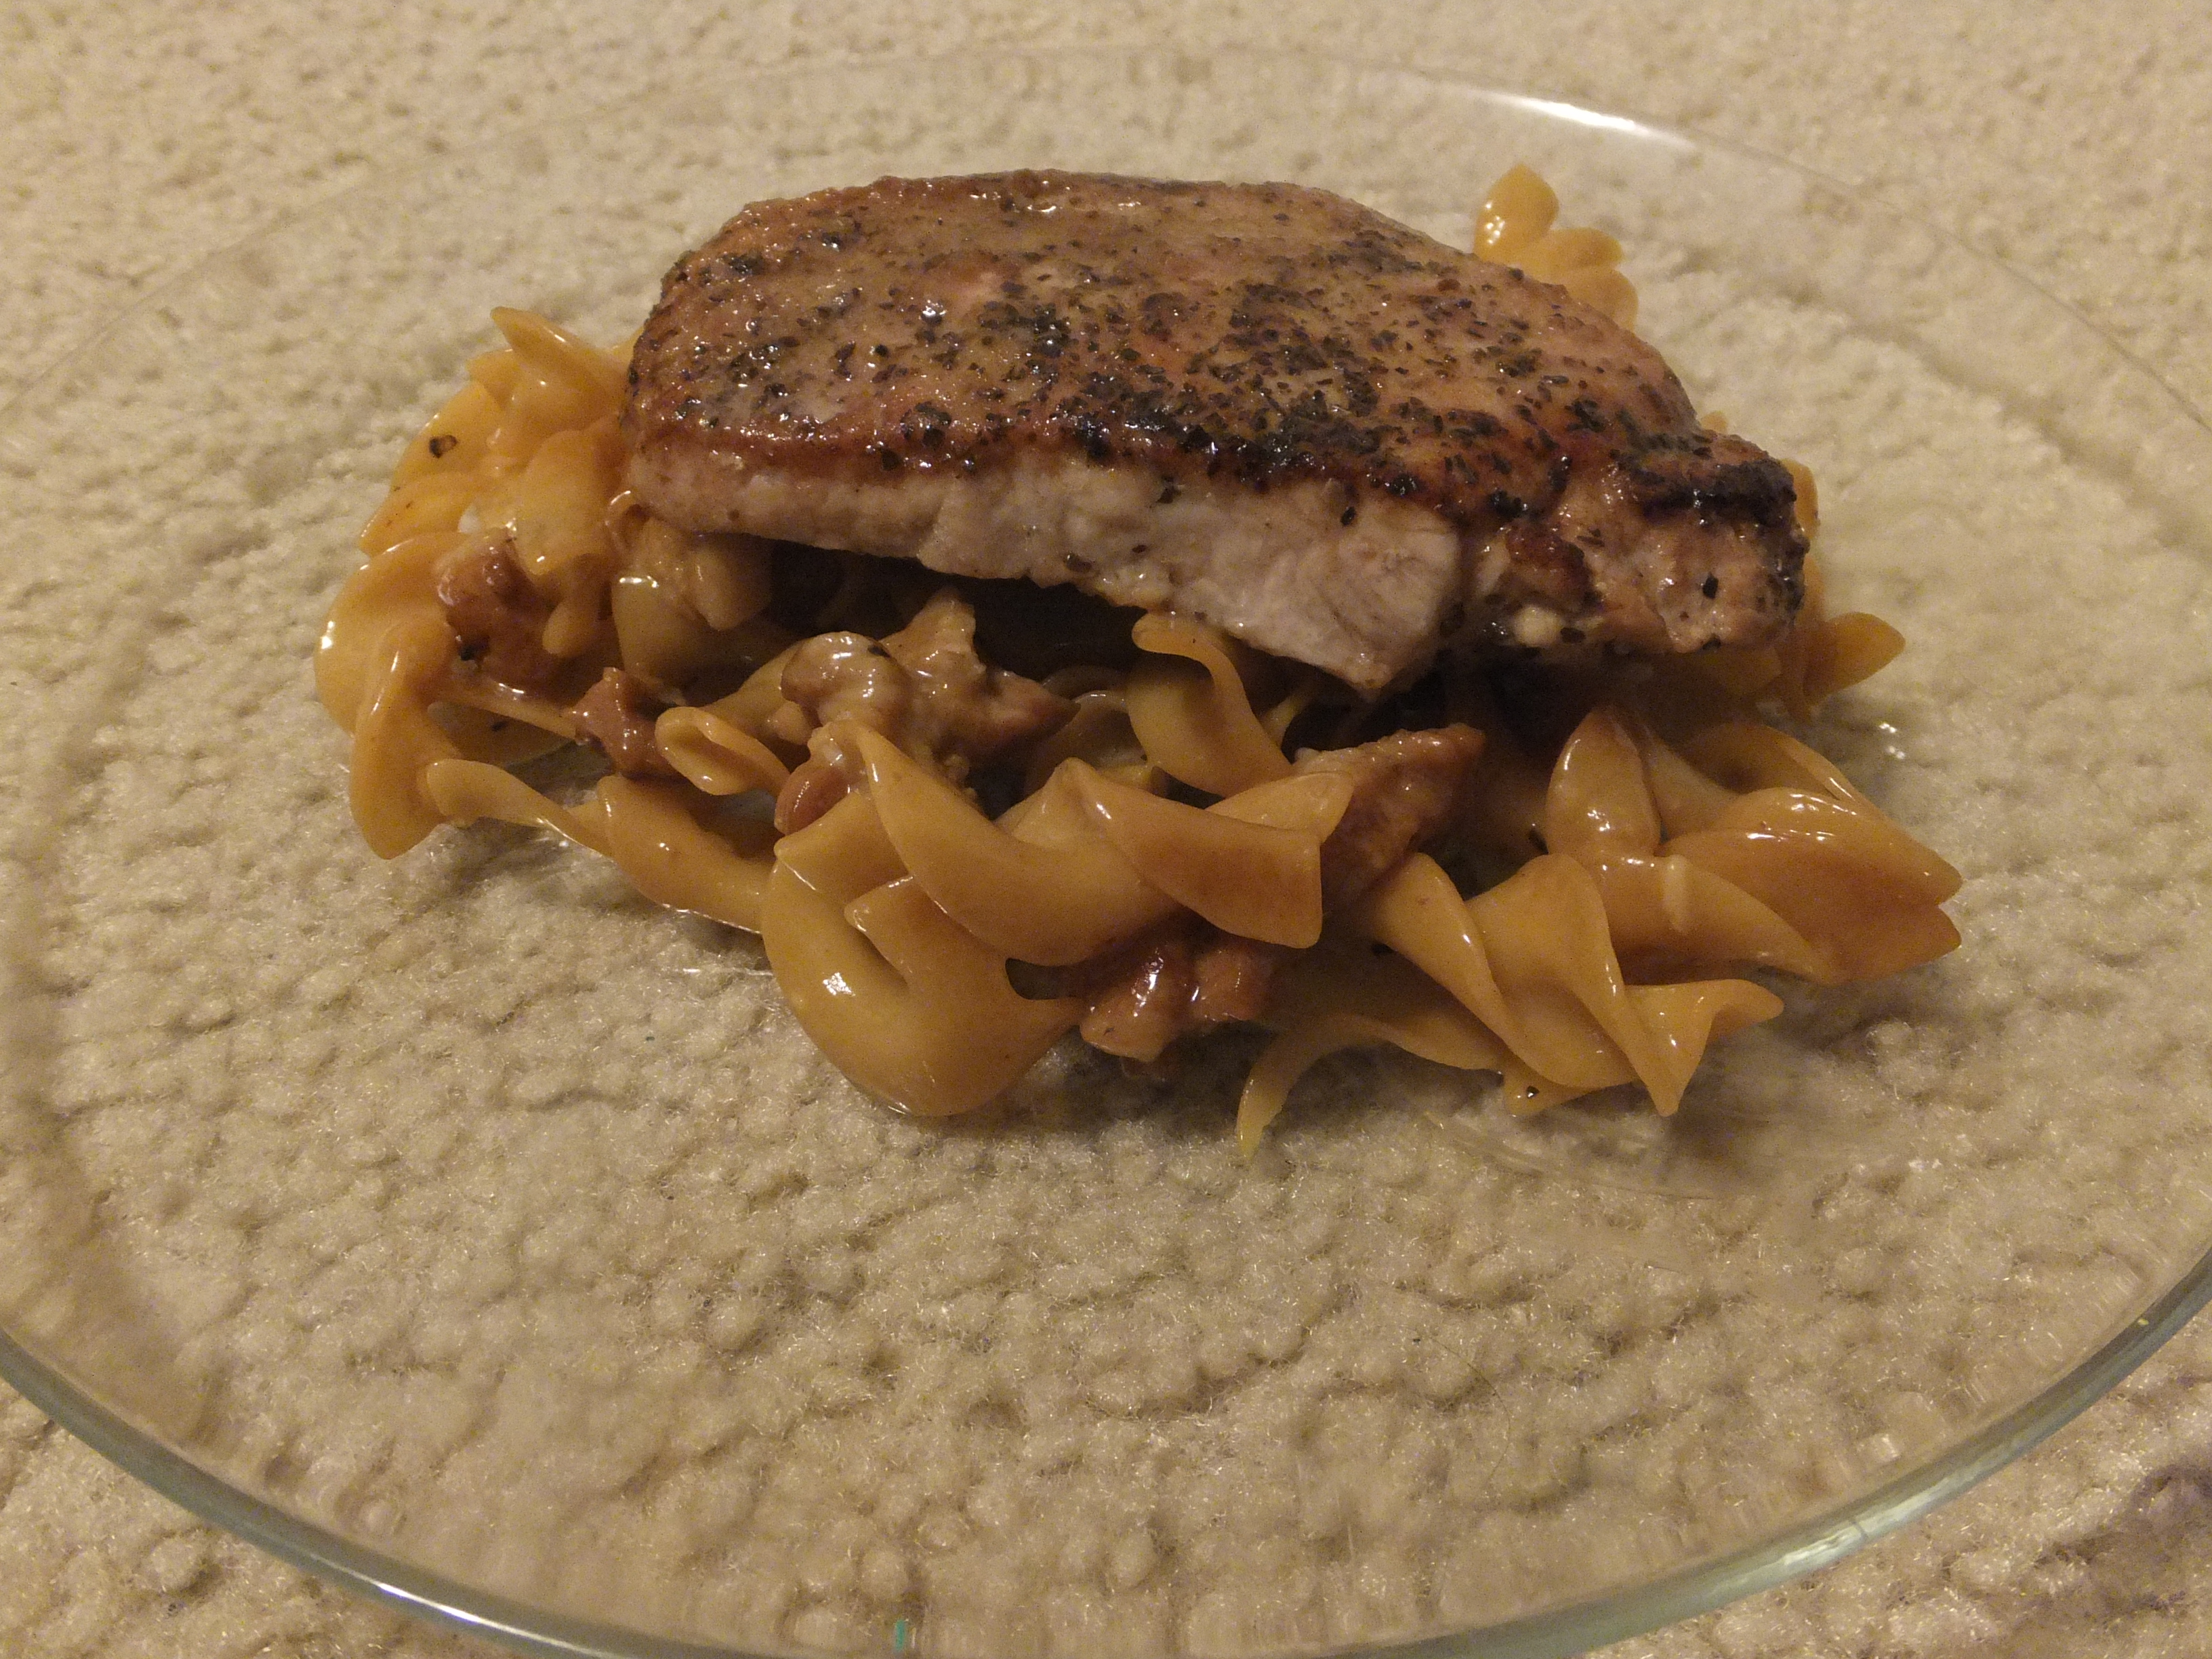
\includegraphics[width=\linewidth,trim=400px 700px 300px 100px, clip=true]{pork_noodles-01.jpeg}
    \end{image}
  \end{images}

  \begin{steps}
  \item Salt the pork for half an hour
  \item Boil the egg noodles
  \item Trim the pork, dice the trimmings
  \item Lightly coat the pork in herbs and flour
  \item Fry the pork on one side in the butter
  \item Flip the pork and braise it in apple juice and water
  \item Remove the pork to rest, but not the trimmings
  \item Add the pepper and noodles to the remaining pork and toss
  \item Beat the egg and mix in the cheese
  \item Stir vigorously while slowly combining the egg and pasta 
  \end{steps}

  \begin{notes}
  \item This was quite good -- I ended up eating both servings.
  \item The noodles ended up sitting a bit too long, I think I just
    need to re-order the noodles later.
  \item A tiny bit of vinegar would probably have been good near the
    end of the gravy.
  \item Mixing the egg and cheese earlier can't hurt
  \end{notes}
\end{recipe}
\end{document}
